\documentclass[conference]{IEEEtran}
\usepackage[spanish]{babel}
\usepackage[utf8]{inputenc}
\usepackage{blindtext, graphicx}
\usepackage{mdwmath}
\usepackage{mdwtab}

\begin{document}
\title{ Thresholding y obtenci\'on del umbral indicado mediante la t\'ecnica de Otsu }
\author{\IEEEauthorblockN{Walter Alejandro Moreno Ram\'irez}
\IEEEauthorblockA{Departamento de Estudios Multidisciplinarios\\
Universidad de Guanajuato\\
Yuriria, Guanajuato\\
Correo: wa.morenoramirez@ugto.mx}}

\maketitle
\renewcommand\abstractname{Abstract}
\begin{abstract}
This article describes what is the meaning of thresholding, what effect it has on an image as well as its applications. It is also described is a way of automatically obtaining the threshold from the histogram of an image, using the Otsu method.. \\\\
\end{abstract}

\begin{IEEEkeywords}
Pixel, histograma, m\'etodo de otsu, umbralizaci\'on, thresholding, threshold, binarizaci\'on, funci\'on, C++, OpenCV.
\end{IEEEkeywords}

\IEEEpeerreviewmaketitle
\section{Introducci\'on}
La \textbf{\emph{umbralizaci\'on}}  o \textbf{\emph{thresholding}} es uno de los m\'etodos m\'as importantes cuando se quiere segmentar una imagen. Para poder aplicarlo es necesario utilizar un valor de referencia, tambi\'en llamado \textbf{\emph{umbral}} a partir del cual se pueda binarizar la imagen, con esto obtenemos una imagen final de \'unicamente dos tonos, blanco y negro. Cuando se binariza la imagen es m\'as f\'acil distinguir los objetos de la imagen y separarlos, lo que se le conoce como segmentaci\'on. \\
La umbralizaci\'on se realiza de acuerdo al siguiente algoritmo.\\\\

\begin{center}
si $I(x,y) > T$  then\\
$g(x,y) = 255$\\
sino\\
$g(x,y) = 0$\\
\end{center}

Donde el valor que sea menor a la referencia se le asigna un nuevo valor de 0 o negro y el valor que sea mayor a la referencia se le asigna el valor de 255 o blanco.\\\\

Se puede obtener el valor de referencia o \textbf{\emph{umbral}} de dos maneras: manual o autom\'atica. Para obtener el umbral de manera manual es necesario obtener el histograma de la imagen, analizar picos, valles y curvaturas con el fin de ubicar el valor central de la imagen, y utilizando como referencia para la umbralizaci\'on.\\
La manera autom\'atica es mediante el m\'etodo de Otsu donde se asume que la imagen contiene dos clases de pixeles (histograma bimodal). Calcula el umbral \'optimo que minimiza la varianza intra-clase y maximiza la varianza inter-clase. Adem\'as de calcular las probabilidades de cada posible clase, y comprueba las varianzas hasta que encuentra la m\'inima dentro de las clases y/o m\'axima entre las clases.\\

\section{Metodolog\'ia}
La ecuaci\'on describe matem\'aticamente como obtener el histograma acumulado de una imagen.\\
\begin{equation}
p_i = \frac{n_i}{N}
\end{equation}
Donde $n_i$ es cada pixel de la imagen y N el total de pixeles.
Las ecuaciones 2 y 3 describen las probabilidades del objeto.
\begin{equation}
\omega_0 = \sum_{i=1}^{K}P_i
\end{equation}
\begin{equation}
\omega_1 = \sum_{i=k+1}^{L}P_i
\omega_1 = 1 - \omega_0
\end{equation}
Las ecuaciones 4 y 5 describen la media para cada clase.
\begin{equation}
\mu_0 = \sum_{i=1}^{k}\frac{iP_i}{\omega_0} 
\end{equation}
\begin{equation}
\mu_1 = \sum_{i=k+1}^{L}\frac{iP_i}{\omega_1}
\end{equation}
La Ecuaci\'on 6 describe la varianza entre clase.
\begin{equation}
\sigma_{B}^{2} = \omega_0\omega_1(\mu_1 - \mu_0)^2
\end{equation}
Se tiene que encontrar el valor de $K$ que maximice la varianza intra clase, y ese valor ser\'a el que utilizaremos como de referencia para la umbralizaci\'on.

Para realizar esta pr\'actica fue necesario crear dos funciones llamas \emph{thresholding} y \emph{otsu}. En la funci\'on \emph{thresholding} se obtiene el histograma de la imagen y, a partir del mismo se realizan los calculos para obtener $\omega_0$, $\omega_1$, $\mu_0$, $\mu_1$ y como resultado final $\sigma_{B}^{2}$ \\
Para realizar las operaciones necesarias se utilizan dos sumas auxiliares. Las cuales nos ayudan para calcular $\mu_0$ y $\mu_1$ de acuerdo al algoritmo de la Figura 3.

\begin{figure}[h]
	\begin{center}
		\setlength{\unitlength}{0.00105in}
		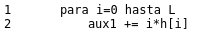
\includegraphics[scale=0.70]{./images/ag1.png}
	\end{center}
	\caption{Algoritmo para obtener la primer suma auxiliar.}
\end{figure}

La Figura 2 muestra el algoritmo que se utiliz\'o para obtener los valores de $\omega_0$, $\omega_1$, $\mu_0$, $\mu_1$ y $\sigma_{B}^{2}$, los cuales son nombrados como w0, w1, u0, u1 y sigmaB respectivamente.\\
El l\'imite del bucle es hasta L que son los niveles de gris de la imagen, en total 255 valores.\\
N es el n\'umero de pixeles total de la imagen.\\
umbral es la variable la cual regresar\'a como valor num\'erico la funci'on \textbf{otsu}.
\begin{figure}[h]
	\begin{center}
		\setlength{\unitlength}{0.00105in}
		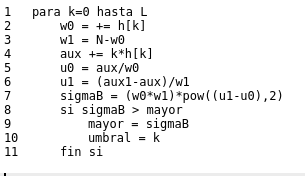
\includegraphics[scale=0.70]{./images/ag2.png}
	\end{center}
	\caption{Algoritmo para obtener los valores de las variables y el umbral \'optimo.}
\end{figure}


%1		para i=0 hasta L
%2			aux1 += i*h[i]

%1 	para k=0 hasta L
%2 		w0 = += h[k]
%3		w1 = N-w0
%4		aux += k*h[k]
%5		u0 = aux/w0
%6		u1 = (aux1-aux)/w1
%7		sigmaB = (w0*w1)*pow((u1-u0),2)
%8 		si sigmaB > mayor
%9			mayor = sigmaB
%10			umbral = k
%11		fin si



\section{Resultados}
Para realizar las pruebas se utilizaron dos imagenes. Una con muchos objetos y poco definidos como lo son \'arboles y otra con pocos objetos y bien definidos.\\
La umbralizaci\'on de la primer imagen y la misma imagen se muestran en la Figura 1.
\begin{figure}[h]
	\begin{center}
		\setlength{\unitlength}{0.00105in}
		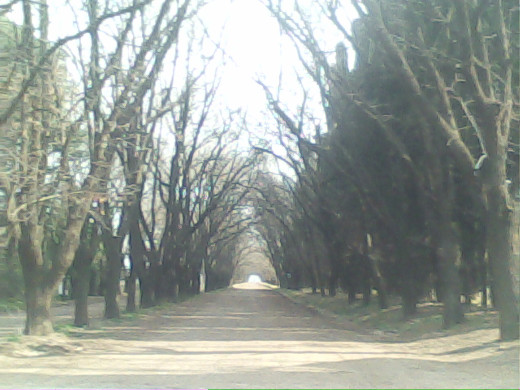
\includegraphics[scale=0.20]{./images/forest.jpg}
		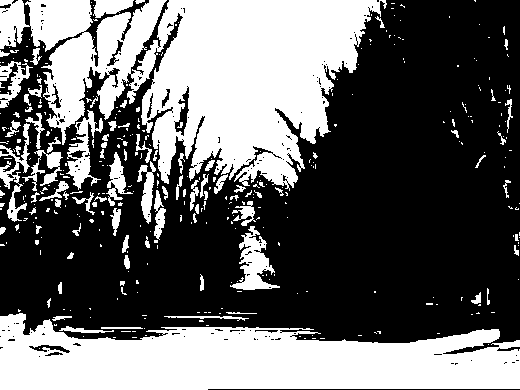
\includegraphics[scale=0.2678]{./images/IMG2.png}
	\end{center}
	\caption{Imagen de un bosque y su umbralizaci\'on.}
\end{figure}

La segunda image y su respectiva imagen umbralizada se muestra en la Figura 2.
\begin{figure}[h]
	\begin{center}
		\setlength{\unitlength}{0.00105in}
		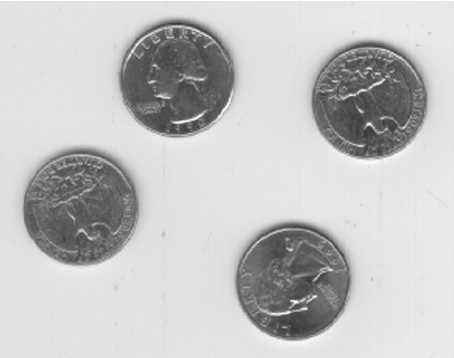
\includegraphics[scale=0.23]{./images/eight.png}
		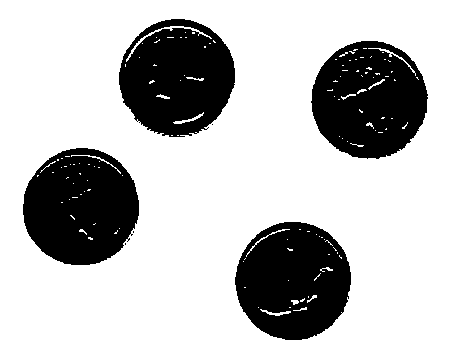
\includegraphics[scale=0.30]{./images/IMG1.png}
	\end{center}
	\caption{Imagen de un bosque y su umbralizaci\'on.}
\end{figure}

\section{Conclusiones}
El m\'etodo de umbralizaci\'on es bastante utilizado y tiene muchas l\'ineas de investigaci\'on. Se puede utilizar para separar objetos, identificarlos y clasificarlos. Ya que existen diferentes m\'etodos para obtener el valor del umbral \'otimo es necesario ya sea utilizar uno ya estudiado o crear uno nuevo de acuerdo a lo que se desee realizar en una imagen o conjunto de im\'agenes.




%\begin{thebibliography}{1}
%    \bibitem{IEEEhowto:kopka}
%    H.~Kopka and P.~W. Daly, \emph{A Guide to \LaTeX}, 3rd~ed.\hskip 1em plus
%      0.5em minus 0.4em\relax Harlow, England: Addison-Wesley, 1999.
%\end{thebibliography}

%\begin{IEEEbiography}[{\includegraphics[width=1in,height=1.25in,clip,keepaspe%ctratio]{picture}}]{John Doe}
%\blindtext
%\end{IEEEbiography}

\end{document}